% ============================================================
% DP Cheat Sheet — Tag reference
% \tp{text}       Plain body paragraph with hanging indent.
% \kp{text}       Hollow-bullet (○) paragraph.
% \fp{text}       Black-bullet paragraph.
% \ap{text}       Arrow (⇒) paragraph.
% \ip{text}       Indented paragraph (all lines at \apmark).
% \is{title}{c}   Italic run-in title + body, \tp-style.
% \mysubsec{t}    Standalone italic subsection label.
% \rb{math}       Boxed display-math recurrence relation.
% code env        Verbatim mono block, compact spacing.
% \mytab{cols}{body}  2/3-width table indented like \tp.
% \defterm{text}  Bold + dashed-underline term definition.
% \prob           Inline-boxed "Problem:" label.
% ============================================================
\documentclass[8pt,letterpaper,twocolumn]{extarticle}
\usepackage[margin=0.2in]{geometry}
\usepackage{amsmath,amssymb,mathtools}
\usepackage{enumitem}
\usepackage{microtype}
\usepackage{listings}
\usepackage{etoolbox}
\usepackage{xcolor}
\usepackage{array}
\usepackage[most]{tcolorbox}
\usepackage{hyphenat}
\usepackage{tikz}
\usetikzlibrary{arrows.meta,positioning,calc}

% ── Global spacing ───────────────────────────────────────────
\linespread{0}
\setlength{\parindent}{0pt}
\setlength{\parskip}{0.6pt}
\setlength{\topsep}{0pt}
\setlength{\partopsep}{0pt}
\setlength{\itemsep}{0pt}
\setlength{\parsep}{0pt}
\setlength{\lineskiplimit}{0pt}
\setlength{\lineskip}{1pt}
\setlength{\jot}{1pt}
\setlength{\fboxsep}{0.5pt}
\setlength{\fboxrule}{0.3pt}
\setlength{\columnsep}{8pt}

% ── Indent lengths ───────────────────────────────────────────
\newlength{\tphang}   \setlength{\tphang}{0.10in}
\newlength{\blistind} \setlength{\blistind}{0.05in}
\newlength{\bmark}    \setlength{\bmark}{0.8em}
\newlength{\apmark}   \setlength{\apmark}{\dimexpr\blistind+\bmark\relax}

% ── Bold + dashed-underline term definition ──────────────────
\newcommand{\defterm}[1]{%
  \smash{\tikz[baseline=(X.base)]{%
    \node[inner sep=0pt,outer sep=0pt] (X) {\textbf{#1}};%
    \draw[dash pattern=on 1.5pt off 1pt,line width=0.4pt]
      ([yshift=-1.2pt]X.base west) -- ([yshift=-1.2pt]X.base east);%
  }}%
}

% ── Inline-boxed "Problem:" label ────────────────────────────
\newcommand{\prob}{%
  \smash{\tikz[baseline=(P.base)]{%
    \node[inner sep=1.5pt,outer sep=0pt,draw,line width=0.4pt] (P)
      {Problem:};%
  }}\hspace{2pt}%
}

% ── Code blocks (continuous grey background via tcolorbox) ───
\definecolor{codebg}{gray}{0.92}

\lstset{
  basicstyle=\ttfamily\normalsize,
  aboveskip=0pt,
  belowskip=0pt,
  xleftmargin=0pt,
  columns=fullflexible,
  keepspaces=true,
  showstringspaces=false,
  breaklines=false,
  frame=none,
}

\newtcblisting{code}{%
  colback=codebg,
  colframe=codebg,
  sharp corners,
  boxrule=0pt,
  left=0.5em,
  right=0pt,
  top=0pt,
  bottom=0pt,
  boxsep=0pt,
  before skip=2pt,
  after skip=2pt,
  listing only,
  listing options={
    basicstyle=\ttfamily\fontsize{7.5}{9}\selectfont,
    aboveskip=0pt,
    belowskip=0pt,
    xleftmargin=0pt,
    columns=fullflexible,
    keepspaces=true,
    showstringspaces=false,
    breaklines=false,
    frame=none,
  },
}

% ── Enumerate ────────────────────────────────────────────────
\setlist[enumerate]{noitemsep,topsep=0pt,parsep=0pt,partopsep=0pt,
  leftmargin=\dimexpr\blistind+\bmark\relax,itemindent=0pt,labelindent=0pt,labelwidth=1em,labelsep=0pt,align=left}

% ── Section / subsection ─────────────────────────────────────
\newcommand{\mysec}[1]{%
  \vspace{\dimexpr5pt-\parskip\relax}%
  \noindent\underline{\smash[b]{#1}}%
  \par\nobreak\ignorespaces}

\newcommand{\mysubsec}[1]{%
  \noindent\textit{#1}\par\nobreak\ignorespaces}

% ── Paragraph macros ─────────────────────────────────────────
\newcommand{\tp}[1]{%
  \hangindent=\tphang\hangafter=1\noindent#1\par}

\newcommand{\kp}[1]{%
  \hangindent=\dimexpr\blistind+\bmark\relax\hangafter=1%
  \noindent\hspace*{\blistind}%
  \makebox[\bmark][l]{\raisebox{0.45ex}{\tiny$\circ$}}#1\par}

\newcommand{\fp}[1]{%
  \hangindent=\dimexpr\blistind+\bmark+\bmark\relax\hangafter=1%
  \noindent\hspace*{\dimexpr\blistind+\bmark\relax}%
  \makebox[\bmark][l]{\raisebox{0.45ex}{\tiny$\bullet$}}#1\par}

\newcommand{\ap}[1]{%
  \hangindent=\dimexpr\blistind+\bmark\relax\hangafter=1%
  \noindent\hspace*{\blistind}%
  \makebox[\bmark][l]{\raisebox{0.3ex}{\footnotesize$\Rightarrow$}}#1\par}

\newcommand{\ip}[1]{%
  {\leftskip=\dimexpr\blistind+\bmark\relax\relax\noindent#1\par}}

\newcommand{\is}[2]{%
  \hangindent=\tphang\hangafter=1\noindent\textit{#1}\ #2\par}

% ── 2/3-width indented table ────────────────────────────────
\newcommand{\mytab}[2]{%
  \par\noindent\hspace*{\tphang}%
  \begin{tabular*}{0.667\linewidth}{#1}%
    #2%
  \end{tabular*}\par}

% ── Recurrence box ───────────────────────────────────────────
\newcommand{\rb}[1]{%
  \par
  \abovedisplayskip=-0.5pt\relax
  \belowdisplayskip=0pt\relax
  \abovedisplayshortskip=-0.5pt\relax
  \belowdisplayshortskip=0pt\relax
  \[\boxed{#1}\]%
  \par
  \global\hangindent=0pt\relax
  \global\hangafter=1\relax
  \global\leftskip=0pt\relax
  \ignorespaces}

\newcommand{\OPT}{\ensuremath{\mathrm{OPT}}}

\pagestyle{empty}
\begin{document}
\fontsize{8}{9.6}\selectfont
\raggedright

%──────────────────────────────────────────────────────────────
\mysec{DP Framework}
%──────────────────────────────────────────────────────────────
\begin{enumerate}
\item Characterize structure of an opt.\ solution
\item Recursively define value of an opt.\ solution
\item Compute value of opt.\ solution bottom-up (fill table)
\item Construct opt.\ solution from computed information
\end{enumerate}

%──────────────────────────────────────────────────────────────
\mysec{Weighted Interval Scheduling}
%──────────────────────────────────────────────────────────────
\tp{Input: set of requests $\{1\ldots n\}$; $i$ starts at $s(i)$, ends at $f(i)$, has weight $w(i)$.
Output: max{-}weight subset of mutually compatible intervals.}
\kp{Sort by finish time: $f_1{\le}\cdots{\le}f_n$. Define $p(j)$ for an interval $j${=}largest index of $i{<}j$ s.t.\ $i$ and $j$ are disjoint.}
\kp{Either $j{\in}O_j$: $\OPT(j){=}w(j){+}\OPT(p(j))$; or $j{\notin}O_j$: $\OPT(j){=}\OPT(j{-}1)$.}
\ap{$\OPT(j)${=}opt.\ value on $\{1\ldots j\}$; $\OPT(0){=}0$.}
\rb{\OPT(j) = \max\bigl(w(j) + \OPT(p(j)),\;\OPT(j - 1)\bigr)}
\mysubsec{Memoized}
\begin{code}
M_Compute_Opt(j):
  if j=0: return 0; if M[j] not empty: return M[j]
  else: M[j]=max(w(j)+M_Compute_Opt(p(j)),M_Compute_Opt(j-1)); return M[j]
\end{code}
\ip{Cannot use bottom{-}up in recursion: may find at ancestor node that whole branch is not optimal.}
\mysubsec{Iterative bottom-up}
\begin{code}
  M[0]=0; for i=1 to n: M[i]=max(M[i-1],w(i)+M[p(i)])
\end{code}
\mysubsec{Find solution at index: $j{\in}O_j$ iff $w(j){+}\OPT(p(j)){\ge}\OPT(j{-}1)$.}
\begin{code}
Find_Solution(j):
  if j>0:
    if w[j]+M[p(j)]>=M[j-1]: {output j; Find_Solution(p(j))}
    else: Find_Solution(j-1)
\end{code}

%──────────────────────────────────────────────────────────────
\mysec{Video Game Problem}
%──────────────────────────────────────────────────────────────
\tp{Stages $0\ldots n$; start with $E_0$; lose $e_i$ landing on stage $i$.
Move costs: walk ({+}1){=}50, jump-1 ({+}2){=}150, jump-2 ({+}3){=}350.
Maximize energy at stage $n$.}
\ap{$\OPT(i)${=}max energy at stage $i$. Recurrence formula:}
\rb{\OPT(i) = \max\!\begin{cases}
\OPT(i{-}1) - 50 - e_i \\
\OPT(i{-}2) - 150 - e_i \\
\OPT(i{-}3) - 350 - e_i
\end{cases}}
\begin{code}
Video_Game(j):
  OPT(0)=E_0; OPT(1)=E_0-50-e_1; OPT(2)=max(E_0-150-e_2,OPT(1)-50-e_2)
  for i=3 to n: use recurrence formula
\end{code}

%──────────────────────────────────────────────────────────────
\mysec{Subset Sum / 0-1 Knapsack}
%──────────────────────────────────────────────────────────────
\tp{Capacity $W$ units of time, have requests $\{1\ldots n\}$ that can be scheduled between $0$ to $W$ each with time $w_i$. Maximize utilization.}
\kp{$\OPT(i)$ over $\{1\ldots i\}$ fails: when $n{\in}O_n$, subproblem has capacity $W{-}w_n$, not $W$, meaning $\OPT(n{-}1)$ are two different values depending on case.}
\ap{$\OPT(i,w)${=}value of opt.\ solution using subset of $\{1\ldots i\}$ with max time $w$.}
\rb{\OPT(i,w) = \begin{cases}
\OPT(i - 1, w) & w < w_i \\
\max(\OPT(i - 1, w),\; w_i + \OPT(i - 1, w - w_i)) & \text{else}
\end{cases}}
\kp{Grid: $(n{+}1){\times}(W{+}1)$ table; rows{=}items $i$, cols{=}capacity $w$.}
\kp{Base row $M[0,w]{=}0$ (no items, zero utilization). Fill row by row: $i{-}1${=}one fewer item in grid; $w$ vs $w{-}w_i$: skip or include item $i$ ($w{-}w_i{<}w_i$ guards negative index). Each row propagate to $M[n][W]$ over all $n$ items. Column $0${=}$0$ units of time, column $1${=}1 unit $\cdots$ W{=}full $W$ units (actual answer).}
\mysubsec{Recurrence}
\begin{code}
Subset_Sum(n,w):
  array M[0][w]=0 for each w=0 to W
  for i=1 to n: for w=0 to W: apply recurrence to M[i][w]
  return M[n][W]
\end{code}
\mysubsec{Bottom-Up}
\begin{code}
Subset_Sum(n,W):
  array M[0..n][0..W]; for w=0 to W: M[0][w]=0
  for i=1 to n: for w=0 to W:
      if w<w_i: M[i][w]=M[i-1][w]
      else: M[i][w]=max(M[i-1][w],w_i+M[i-1][w-w_i])
  return M[n][W]
\end{code}
\is{0/1 Knapsack:}{Items have weight $w_i$ value $v_i$. Replace $w_i{\to}v_i$ in max branch.}
\ap{$\OPT(i,w)${=}max value using $\{1\ldots i\}$, capacity $w$.}
\rb{\OPT(i,w) = \max\bigl(\OPT(i - 1, w),\; v_i + \OPT(i - 1, w - w_i)\bigr)}
\kp{Runtime: $\theta(nW)${=}pseudo-polynomial. Need $\log_2 W$ bits to represent $W$.}
\kp{Rewriting: $nW{=}n{\cdot}2^{\log_2 W}$, exponential in input size ${\Rightarrow}$ NOT polynomial.}
\tp{Polynomial: $T$ poly in input length. Pseudo-: $T$ poly in numeric value of input.}

%──────────────────────────────────────────────────────────────
\mysec{Sequence Alignment}
%──────────────────────────────────────────────────────────────
\tp{Given $X{=}x_1\cdots x_m$, $Y{=}y_1\cdots y_n$ (e.g.\ DNA), find minimum-cost alignment.
A matching is a set of ordered pairs with the property that each item occurs at most once.
An alignment is a matching with no crossing pairs: if $(i,j),(i',j'){\in}M$ with $i{<}i'$, then $j{<}j'$.}
\kp{SEASIDE vs.\ DISEASE: a perfect matching exists but pairs cross ${\Rightarrow}$ not an alignment, not similar.}
\kp{Cost: gap penalty $\delta$ per gap; mismatch cost $\alpha_{pq}$ with $\alpha_{pp}{=}0$. Similarity${=}$min-cost alignment of $X$ and $Y$.}
\ap{$\OPT(i,j)${=}min-cost alignment of $x_1\cdots x_i$ and $y_1\cdots y_j$. Either $(x_m,y_n){\in}M$ (match/mismatch); $x_m$ unmatched (gap in $Y$); or $y_n$ unmatched (gap in $X$).}
\rb{\OPT(i,j) = \min\!\begin{cases}
\OPT(i{-}1, j{-}1) + \alpha_{x_i y_j}\\
\OPT(i{-}1, j) + \delta\\
\OPT(i, j{-}1) + \delta
\end{cases}}
\begin{code}
  OPT(i,0)=i*delta; OPT(0,j)=j*delta
  for i=1 to m: for j=1 to n: apply recurrence
\end{code}
\kp{Runtime: $O(mn)$. Space: $O(mn)$.}

%──────────────────────────────────────────────────────────────
\mysec{Sequence Alignment (Memory-Efficient D\&C)}
%──────────────────────────────────────────────────────────────
\tp{Split $X$ at midpoint into $X_L$ and $X_R$. Key: find optimal split point $k^*$ in $Y$.}
\kp{Forward DP with $Y$ on rows, $X_L$ on columns: init column $0$ as $k\delta$ for row $k$ (aligning none of $X_L$ against $y_1\cdots y_k$ costs $k$ gaps).}
\fp{Define $\mathrm{fwd}$ as the last column as a 1D array.}
\fp{Last column gives $\mathrm{fwd}[k]${=}optimal cost of aligning $X_L$ with $y_1\cdots y_k$ $\forall\; 0{\le}k{\le}n$ (cumulative number of edits since first entry to $k$).}
\fp{$\mathrm{fwd}[0]{=}m_L\delta$ ($X_L$ against none of $Y$); $\mathrm{fwd}[n]{=}$opt.\ cost to align $X_L$ $\forall$ $Y$.}
\kp{Backward DP on $(Y^{\mathrm{rev}}$, $X_R^{\mathrm{rev}})$: init column $0$ as $(n{-}k)\delta$ for row $(n{-}k)$ (aligning none of $X_R$ against $y_{n-k}\cdots y_n$ costs $(n{-}k)$) gaps.}
\fp{Last column gives $\mathrm{bwd}[k]${=}opt.\ cost of aligning $X_R$ with $y_{n-k}\cdots y_n$.}
\fp{$\mathrm{bwd}[n]{=}$opt.\ cost of aligning $X_R$ with all of $Y$.}
\kp{Optimal split: find $k^*$ s.t.\ $\mathrm{fwd}[k^*]{+}\mathrm{bwd}[n{-}k^*]$ is minimized over $0{\le}k{\le}n$. Recurse on $(X_L,Y[1..k^*])$ and $(X_R,Y[k^*{+}1..n])$.}
\begin{code}
MemEff(X,Y):
  m=|X|,n=|Y|
  if m<=2 or n<=2: return StandardDP(X,Y)
  mid=floor(m/2),X_L=X[1..mid],X_R=X[mid+1..m]
  fwd=LastCol(X_L,Y),bwd=LastCol(reverse(X_R),reverse(Y))
  best_k=0,best=fwd[0]+bwd[n]
  for k=1 to n:
    if fwd[k]+bwd[n-k]<best: best=fwd[k]+bwd[n-k],best_k=k
  return MemEff(X_L,Y[1..best_k]) + MemEff(X_R,Y[best_k+1..n])

StandardDP(X,Y):
  m=|X|,n=|Y|; for i=0 to m: OPT[i,0]=i*d; for j=0 to n: OPT[0,j]=j*d
  for i=1 to m: for j=1 to n:
    OPT[i,j]=min(a(x_i,y_j)+OPT[i-1,j-1],d+OPT[i-1,j],d+OPT[i,j-1])
  return OPT
\end{code}
\ip{Each D\&C level does $O(mn)$ work total across all subproblems (halving each time: $mn{+}mn/2{+}\cdots{\le}2mn$). Overall: Time $\Theta(mn)$, Space $O(m{+}n)$.}

%──────────────────────────────────────────────────────────────
\mysec{Matrix Chain Multiplication}
%──────────────────────────────────────────────────────────────
\tp{Given $n$ dense matrices $A_1\cdots A_n$, find multiplication order to min.\ operations.}
\kp{Key: last multiplication\ of $A_i\cdots A_j$ must involve the multiplication of results of $(A_i\cdots A_k){\cdot}(A_{k+1}\cdots A_j)$ where $i{\le}k{<}j$.}
\ap{$\OPT(i,j)${=}optimal cost for $A_i\cdots A_j$; $\OPT(i,i){=}0$. $R_i${=}rows of $A_i$; $C_k${=}cols of $A_k$; $C_j${=}cols of $A_j$.}
\rb{\OPT(i,j) = \min_{i \le k < j}\bigl\{\OPT(i,k) + \OPT(k{+}1, j)\bigr\} + R_i C_k C_j}
\ip{Time: $O(n^3)$.}

%──────────────────────────────────────────────────────────────
\mysec{Bellman-Ford (Shortest Paths)}
%──────────────────────────────────────────────────────────────
\tp{Directed graph, possibly negative weights. Negative cycle with path to $t$ implies dist${=}{-\infty}$. Find shortest s-t path.}
\kp{If no negative cycles: shortest path is simple (loop-free), at most $n{-}1$ edges.}
\ap{$\OPT(i,v)${=}min cost of $v{\to}t$ path using ${\le}i$ edges. Goal: find $\OPT(n{-}1,s)$.}
\rb{\OPT(i,v) = \min\!\begin{cases}
\OPT(i{-}1, v) & \text{$\le i$ edges} \\
\min_{w \in \mathrm{Adj}(v)}\!\bigl(\OPT(i{-}1, w) + c_{vw}\bigr) & \text{else}
\end{cases}}
\begin{code}
Bellman_Ford(G,s,t):
  n=number of nodes in G
  OPT(0,t)=0,OPT(0,v)=infty
  for i=1 to n-1: for v in V in any order: use recurrence formula
\end{code}
\ip{Worst-case: $O(n^3)$. Tight bound: $\Theta(mn)$.}
\is{Variant:}{Reuse one array. Updating $t{\to}s$ along a path takes 2 passes, but $s{\to}t$ needs $n{-}1$. Key: first visit nodes closer to $t$ in no.\ of edges.}
\mysubsec{Negative cycle detection}
\kp{If $\OPT(n,v){<}\OPT(n{-}1,v)$ for any $v$: negative cycle reachable to $t$.}
\kp{Problem: cycle with no path to $t$ keeps $\infty$ distances, never detected.}
\kp{Fix: add super-sink $t^*$ with 0-cost edges from every node to $t^*$. Run Bellman-Ford to $t^*$. Now every negative cycle can reach $t^*$, so extra-iteration catches them. 0-cost edges to $t^*$ only checks reachability.}
\mysubsec{Bellman-Ford vs.\ Dijkstra}
\mytab{@{}l@{\extracolsep{\fill}}l@{\hspace{1.5em}}l@{}}{%
 & Bellman-Ford & Dijkstra \\
Time & $O(mn)$ & $O(m\log n)$ \\
Neg.\ weights & yes & no \\
}

%──────────────────────────────────────────────────────────────
% NETWORK FLOW
%──────────────────────────────────────────────────────────────
\mysec{Network Flow}
%──────────────────────────────────────────────────────────────
\tp{A \defterm{flow network} is a directed graph $G{=}(V,E)$ with: (1) each edge $e$ having non-negative int capacity $c_e$; (2) a single source $s{\in}V$; (3) a single sink $t{\in}V$.}
\kp{Assumptions: no edges enter $s$ or leave $t$; at least one edge incident to each node ($e{\ge}v/2$ so $O(e{+}v){=}O(e)$); all capacities are integers.}
\mysubsec{Flow $f(e)$ properties}
\kp{Capacity constraint: for each $e{\in}E$, $0{\le}f(e){\le}c_e$.}
\kp{Conservation of flow: for each $v{\in}V\setminus\{s,t\}$, $\sum_{e\;\text{into}\;v}f(e){=}\sum_{e\;\text{out of}\;v}f(e)$.}
\ap{Value of steady-state flow (no transient/burst): $v(f){=}\sum_{e\;\text{out of}\;s}f(e)$.}

%──────────────────────────────────────────────────────────────
\mysec{Max Flow Problem}
%──────────────────────────────────────────────────────────────
\tp{Given flow network $G$, find $s$-$t$ flow with max value. Greedy approaches fail. Create Residual graph $G_f$ with same nodes as $G$. For each edge $e$ in $G$:}
\kp{$f(e){=}0$: $G_f$ has 1 forward edge with cap.\ $c_e$ (does not change if unused).}
\kp{$f(e){=}c_e$: $G_f$ has 1 backward edge with cap.\ $c_e$ (reverse direction).}
\kp{$0{<}f(e){<}c_e$: $G_f$ has 1 fwd edge (cap.\ $c_e{-}f(e)$) and 1 bwd edge (cap.\ $f(e)$).}

%──────────────────────────────────────────────────────────────
\mysec{Augmenting Paths \& Ford-Fulkerson}
%──────────────────────────────────────────────────────────────
\tp{If $P$ is a simple $s$-$t$ path in $G_f$, bottleneck$(P)$ is the min residual capacity of any edge on $P$. High-level strategy:}
\ip{Find $s$-$t$ path $P$ in $G_f$; find bottleneck$(P)$ for path; push flow along $P$ equal to bottleneck; update $G_f$; repeat until no $s$-$t$ path exists.}
\begin{code}
Augment(f,C,P):
  b=bottleneck(P)
  for each edge (v,u) in P:
    if (v,u) is forward edge: increase f(e) by b
    else (v,u) is backward edge: let e=(u,v),decrease f(e) by b
  return f'
\end{code}
\mysubsec{Ford-Fulkerson Algorithm}
\begin{code}
MaxFlow(G,s,t,C):
  init f(e)=0 for all e in G
  while there is s-t path in G_f:
    let P be simple s-t path in G_f,f'=Aug(f,C,P),f=f',update G_f
  return f
\end{code}

%──────────────────────────────────────────────────────────────
\mysec{Cuts \& Max-Flow Min-Cut}
%──────────────────────────────────────────────────────────────
\tp{$\defterm{Capacity}$ of cut: $c(A,B){=}\sum_{e\;\text{out of}\;A}c_e$. Only count $A{\to}B$, not $B{\to}A$.}
\tp{Let $f$ be any $s$-$t$ flow and $(A,B)$ be any $s$-$t$ cut, then $v(f){=}f^{\text{out}}(A){-}f^{\text{in}}(A)$.}
\ap{$v(f){\le}f^{\text{out}}(A){\le}\sum_{e\;\text{out of}\;A}c_e{=}c(A,B)$.}
\kp{Weak duality: $v(f){\le}c(A,B)$, so max flow is bounded by cap of $\forall$ $s$-$t$ cuts.}
\tp{\defterm{Max-Flow Min-Cut Theorem:} max value of an $s$-$t$ flow (flow passing from $s{\to}t$) equals min capacity of an $s$-$t$ cut (i.e., smallest total weight of edges which if removed would disconnect source from sink).}
\ap{Lemma: if there is no $s$-$t$ path in $G_{Ford}$, then $\exists$ $s$-$t$ cut $(A^*,B^*){\in}G$ s.t.\ $v(f){=}c(A^*,B^*)$ and has the min capacity of any $s$-$t$ cut in $G$.}
\kp{Min cut is not always unique. E.g., $s{\to}{\cdot}{\to}{\cdot}{\to}t$.}
\kp{Check uniqueness: find min-cut closest to $s$ and min-cut closest to $t$. If they are the same cut, min-cut must be unique.}

%──────────────────────────────────────────────────────────────
\mysec{Scaling Ford-Fulkerson}
%──────────────────────────────────────────────────────────────
\tp{Idea: only augment along paths with ``large'' residual capacity.}
\begin{code}
Scaling_MaxFlow(G,s,t,C):
  f(e)=0 for all e; delta=largest power of 2<=max cap of one edge out of s
  while delta>=1:
    while there is s-t path in G_f(delta):
      P=simple s-t path in G_f(delta)
      f'=Augment(f,C,P),f=f',update G_f(delta)
    delta=delta/2
  return f
\end{code}

%──────────────────────────────────────────────────────────────
\mysec{Edmonds-Karp \& Other Algorithms}
%──────────────────────────────────────────────────────────────
\tp{Same as Ford-Fulkerson, but always use augmenting path that is the shortest path (BFS) with remaining capacity. Running time: $O(nm^2)$, strongly poly.}
\mysubsec{Max-flow algorithm comparison}
\mytab{@{}l@{\extracolsep{\fill}}l@{\hspace{0.8em}}l@{}}{%
Algorithm & Time & Type \\
Ford-Fulkerson & $O(Cm)$ & pseudo-poly \\
Scaling F-F & $O(m^2\log C)$ & weakly poly \\
Edmonds-Karp & $O(nm^2)$ & strongly poly \\
}

%──────────────────────────────────────────────────────────────
% NETWORK FLOW APPLICATIONS
%──────────────────────────────────────────────────────────────

\mysec{Bipartite Matching via Max Flow}
%──────────────────────────────────────────────────────────────
\tp{\defterm{Bipartite graph} $G{=}(V,E)$: undirected graph that nodes can be partitioned as $V{=}X{\cup}Y$ s.t.\ every edge $e{\in}E$ connects one node in $X$ and one in $Y$.}
\tp{A \defterm{matching} $M$ in $G$ is a subset $M{\subseteq}E$ s.t.\ each node appears in at most one edge in $M$. \defterm{Max-size} match: add new edge will make a node appear twice.}
\tp{\prob Given bipartite graph $G$, find largest possible matching in $G$. Plan: design flow-net $G'$ that has flow value $v(f){=}k$ iff $\exists$ a matching of size $k$ in $G$.}
\begin{center}
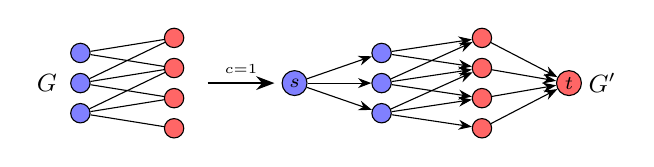
\begin{tikzpicture}[>=Stealth, scale=0.85,
  xn/.style={circle,draw,fill=blue!50,inner sep=0pt,minimum size=7pt},
  yn/.style={circle,draw,fill=red!60,inner sep=0pt,minimum size=7pt},
  sn/.style={circle,draw,fill=blue!50,inner sep=1pt,minimum size=9pt,font=\bfseries\scriptsize},
  tn/.style={circle,draw,fill=red!60,inner sep=1pt,minimum size=9pt,font=\bfseries\scriptsize}]
  %--- G (left) ---
  \node[font=\small] at (-0.5, 0) {$G$};
  \node[xn] (gx1) at (0, 0.45)  {};
  \node[xn] (gx2) at (0, 0)    {};
  \node[xn] (gx3) at (0,-0.45)  {};
  \node[yn] (gy1) at (1.4, 0.675) {};
  \node[yn] (gy2) at (1.4, 0.225) {};
  \node[yn] (gy3) at (1.4,-0.225) {};
  \node[yn] (gy4) at (1.4,-0.675) {};
  \draw (gx1)--(gy1); \draw (gx1)--(gy2);
  \draw (gx2)--(gy1); \draw (gx2)--(gy2); \draw (gx2)--(gy3);
  \draw (gx3)--(gy2); \draw (gx3)--(gy3); \draw (gx3)--(gy4);
  %--- G' (right) ---
  \pgfmathsetmacro{\ox}{3.2}
  \node[sn] (s) at (\ox+0,    0)    {$s$};
  \node[xn] (x1) at (\ox+1.3, 0.45)  {};
  \node[xn] (x2) at (\ox+1.3, 0)    {};
  \node[xn] (x3) at (\ox+1.3,-0.45)  {};
  \node[yn] (y1) at (\ox+2.8, 0.675) {};
  \node[yn] (y2) at (\ox+2.8, 0.225) {};
  \node[yn] (y3) at (\ox+2.8,-0.225) {};
  \node[yn] (y4) at (\ox+2.8,-0.675) {};
  \node[tn] (t) at  (\ox+4.1, 0)    {$t$};
  \node[font=\small] at (\ox+4.6, 0) {$G'$};
  \foreach \x in {x1,x2,x3} \draw[->] (s)--(\x);
  \draw[->] (x1)--(y1); \draw[->] (x1)--(y2);
  \draw[->] (x2)--(y1); \draw[->] (x2)--(y2); \draw[->] (x2)--(y3);
  \draw[->] (x3)--(y2); \draw[->] (x3)--(y3); \draw[->] (x3)--(y4);
  \foreach \y in {y1,y2,y3,y4} \draw[->] (\y)--(t);
  %--- Arrow between G and G' ---
  \draw[->,thick] (1.9,0) -- (2.9,0);
  \node[font=\tiny,above] at (2.4,0) {$c{=}1$};
\end{tikzpicture}
\end{center}
\mysubsec{Solution}
\tp{Find max flow $f$ in $G'$. Edges with flow between $(X,Y)$ correspond to max-size matching $M$ in $G$. Prove $G'$ has flow of value $k$ iff $G$ has matching of size $k$.}
\kp{If $\exists$ matching of size $k$ in $G$: each independent $s$-$t$ path gives $c{=}1$, so there is an $s$-$t$ flow of $v(f){=}k$ in $G'$.}
\kp{If flow $v(f){=}k$ in $G'$: must be $k$ edges on cut $(A,B)$ between $(X,Y)$ that carry flow. These $k$ edges cannot share any node ${\rightarrow}$ matching of size $k$ in $G$.}
\tp{Ford-Fulkerson is $O(Cm)$. Since all $c_e{=}1$, $C{=}O(n)$. $T{=}O(mn)$, strong poly.}

%──────────────────────────────────────────────────────────────
\mysec{Edge-Disjoint Paths}
%──────────────────────────────────────────────────────────────
\tp{A set of paths is \defterm{edge-disjoint} if they do not share any edge. \prob given directed $G{=}(V,E)$ and $s,t{\in}V$, find max number of edge-disjoint $s$-$t$ paths.}
\ap{Design FN $G'$ as $G$ iff {$\exists$} $k$ edge-disjoint $s$-$t$ paths in $G$. Set $c_e{=}1$ $\forall$ edges (already has $s,t$), remove $t$-$s$ paths and do not count intermediate paths.}
\mysubsec{Solution}
\tp{Find max flow $f$ in $G'$. $v(f)$ equals max number of edge-disjoint $s$-$t$ paths, so $f$ identifies edges on these paths. Proof: show there are $k$ edge-disjoint paths in $G$ iff there exists a flow of value $k$ in $G'$.}
\kp{If have $k$ edge-disjoint paths in $G$, $\exists$ flow of value $k$ in $G'$ ${\because}$ each path $c{=}1$.}
\kp{Flow of value $k$ in $G'$: use conservation of flow to follow each unit from $s{\rightarrow}t$; remove all edges on that path from $G'$, repeat $k$ times to find $k$ edge-disjoint $s$-$t$ paths in $G$ since there are $k$ units of flow leaving $s$.}
\mysubsec{Handling flow cycles}
\ip{Since there are ${\ge}2$ units of flow entering $v$, there must be ${\ge}2$ leaving. Remove cycle edges; use the other outgoing edge to continue toward $t$.}
\mysubsec{Flow cycles in undirected graphs}
\ip{Replace each undirected edge with 2 directed edges in opposite directions ($c{=}1$ each). \prob two paths will use $e{=}\{u,v\}$ in opposite directions.}
\ap{Fix: before extracting $s$-$t$ paths, remove all flow cycles on single edges.}
\tp{Runtime with Ford-Fulkerson: $O(mn)$ (same as bipartite matching).}

%──────────────────────────────────────────────────────────────
\mysec{Node-Disjoint Paths}
%──────────────────────────────────────────────────────────────
\tp{A set of paths is \defterm{node-disjoint} if paths between two nodes share no common node (except $s$ and $t$). Given directed $G{=}(V,E)$ and $s,t{\in}V$, find max number of node-disjoint $s$-$t$ paths.}
\ap{For each node $v{\in}V\setminus\{s,t\}$: split $v$ into $v_{\text{in}}$ and $v_{\text{out}}$ connected by a single edge $(v_{\text{in}},v_{\text{out}})$ with $c{=}1$. All incoming edges of $v$ go to $v_{\text{in}}$; all outgoing edges of $v$ leave from $v_{\text{out}}$. Set $c{=}1$ for all other edges.}
\begin{center}
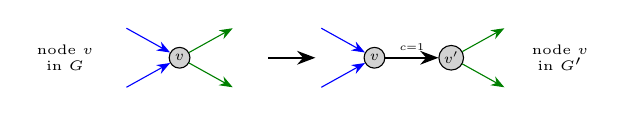
\begin{tikzpicture}[>=Stealth, scale=0.75, every node/.style={transform shape},
  nd/.style={circle,draw,fill=gray!35,inner sep=1pt,minimum size=10pt,font=\scriptsize}]
  % Left: original
  \node[nd] (v) at (0,0) {$v$};
  \draw[<-,blue] (v) -- ++(-0.9,0.5);
  \draw[<-,blue] (v) -- ++(-0.9,-0.5);
  \draw[->,green!50!black] (v) -- ++(0.9,0.5);
  \draw[->,green!50!black] (v) -- ++(0.9,-0.5);
  \node[transform shape=false,font=\tiny,align=center,anchor=east] at (-1.3,0) {node $v$\\in $G$};
  % Arrow
  \draw[->,thick] (1.5,0) -- (2.3,0);
  % Right: split
  \node[nd] (vin) at (3.3,0) {$v$};
  \node[nd] (vout) at (4.6,0) {$v'$};
  \draw[->,thick] (vin)--(vout) node[midway,above,font=\tiny]{$c{=}1$};
  \draw[<-,blue] (vin) -- ++(-0.9,0.5);
  \draw[<-,blue] (vin) -- ++(-0.9,-0.5);
  \draw[->,green!50!black] (vout) -- ++(0.9,0.5);
  \draw[->,green!50!black] (vout) -- ++(0.9,-0.5);
  \node[transform shape=false,font=\tiny,align=center,anchor=west] at (5.8,0) {node $v$\\in $G'$};
\end{tikzpicture}
\end{center}
\tp{(General plan same as the previous problem.)}

%──────────────────────────────────────────────────────────────
\mysec{Circulation}
%──────────────────────────────────────────────────────────────
\tp{A \defterm{circulation network} is a directed graph $G{=}(V,E)$ where each edge $e$ has capacity $c_e{\ge}0$ and each node $v{\in}V$ has a demand $d_v$.}
\fp{$d_v{>}0$: node $v$ is a sink (demands $d_v$ flow).}
\fp{$d_v{<}0$: node $v$ is a source (supplies $|d_v|$ flow).}
\fp{$d_v{=}0$: neither sink nor source.}
\mysubsec{Circulation $f(e)$ properties}
\kp{Capacity: for each $e{\in}E$, $0{\le}f(e){\le}c_e$.}
\kp{Demand: $\forall$ node $v$, $\sum_{e\ into\ v}f(e){-}\sum_{e\ out of\ v}f(e){=}f^{\text{in}}(v){-}f^{\text{out}}(v){=}d_v$.}
\kp{If feasible circulation exists, then $\sum_v d_v{=}0$.}
\ip{Proof: $\sum_v d_v{=}\sum_v(f^{\text{in}}(v){-}f^{\text{out}}(v))$. Each edge $e$ contributes ${+}f(e)$ to one node's $f^{\text{in}}$ and ${-}f(e)$ to another's $f^{\text{out}}$, so all terms cancel ($\sum_v d_v=0$).}
\tp{\prob Given a CN $G$ with demands $\{d_v\}$, $\exists$ feasible circulation in $G$?}
\ap{Reduction to max-flow: make $G'$ keep all edges/caps from $G$. Add super-source $s^*$ and super-sink $t^*$:}
\kp{For each node $v$ with $d_v{<}0$ (source): add edge $(s^*,v)$ with cap $|d_v|$.}
\kp{For each node $v$ with $d_v{>}0$ (sink): add edge $(v,t^*)$ with cap $d_v$.}
\tp{Find max flow $f$ in $G'$ with total demand $D$.}
\fp{$v(f){<}D$: no feasible circulation exists in $G$.}
\fp{$v(f){>}D$: impossible (cuts closest to $s^*$ and $t^*$ each have capacity $D$).}
\fp{$v(f){=}D$: feasible circulation exists; flow on original edges (i.e., strip edges from $s^*$ and to $t^*$) gives valid circulation.}

\mysubsec{Reduction proof-of-correctness}
\begin{enumerate}
    \item If {$\exists$} circ.\ $f$ with demands $\{d_v\}$ in $G$, there is max flow of value $D$ in $G'$. \\ If $G$ has circulation satisfying all demands, the net flow absorbed/produced by each demand node can be rerouted thru super-source/sink edges. Each node with $d_v{>}0$ was receiving $d_v$ net flow, which now comes from $(s^*,v)$, so all $s^*$ edges are saturated. Thus max flow in $G'$ achieves $D{=}\sum_{d_v>0}d_v$.
    \item If {$\exists$} max flow of value $D$ in $G'$, there is feasible circulation $f$ with {$\{d_v\}$} in $G$. \\ If {$v(f)$} in $G'${=}$D$, every $e{=}(s^*,v)$ is saturated, i.e. demand is fully supplied. Remove $s^*,t^*$ and redirect flow back to original demand gives $f{\in} G$.
\end{enumerate}

%──────────────────────────────────────────────────────────────
\mysec{Circulation with Lower Bounds}
%──────────────────────────────────────────────────────────────
\tp{$G{=}(V,E)$ where edge $e$ also has lower bound $\ell_e$ so $\ell_e{\le}f(e){\le}c_e$. Demand, source, and sink are same. \prob is there a feasible circ. in G?}
\ap{Reduce feasible circulation with lower bounds to feasible circulation.}
\kp{Push initial flow $f_0$ where $f_0(e){=}\ell_e$ through $G$ to create flow imbalance $L_v$ based on $f_0$ at each node $v$ (find $f_0$ to satisfy all $\ell_e$'s):}
\rb{L_v = \sum_{e\;\text{into}\;v}\!\ell_e \;-\; \sum_{e\;\text{out of}\;v}\!\ell_e}
\kp{Construct $G'$ with $c'_e{=}c_e{-}\ell_e$, $\ell'_e{=}0$, and $d'_v{=}d_v{-}L_v$.}
\kp{Find feasible circ.\ $f_1$ in $G'$ (using max-flow reduction \& remaining capacity). If none exists, no feasible circulation in $G$. Otherwise, feasible $G{=}f_0{+}f_1$.}

%──────────────────────────────────────────────────────────────
\mysec{Survey Design Problem}
%──────────────────────────────────────────────────────────────
\tp{Input: which customer bought which product; $\forall$ customer $i$, ask min/max questions $(m_i,\ell_i)$; $\forall$ product $j$, ask min/max questions $(m_j,\ell_j)$.}
\ap{Reduce to circulation with lower bounds.}
\kp{Build bipartite FN with source $s$, sink $t$, customer and product nodes:}
\fp{$s{\to}i$: capacity $[\,\ell_i,\;m_i\,]$ {$\cdots$} bounds on questions per customer.}
\fp{$i{\to}j$ ($i$ bought $j$): cap $[\,0,\;1\,]$ {$\cdots$} ask {$\le$}1 ques.\ per product per customer.}
\fp{$j{\to}t$: capacity $[\,\ell_j,\;m_j\,]$ {$\cdots$} bounds on questions per product.}
\begin{center}
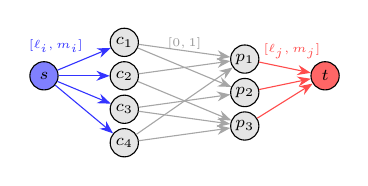
\begin{tikzpicture}[>=Stealth, scale=0.85, every node/.style={transform shape},
  nd/.style={circle,draw,fill=gray!20,inner sep=1pt,minimum size=12pt,font=\scriptsize}]
  \node[nd,fill=blue!50] (s) at (0,0) {$s$};
  \foreach \i [evaluate=\i as \y using {0.5-(\i-1)*0.5}] in {1,...,4} {
    \node[nd] (c\i) at (1.2, \y) {$c_\i$};
  }
  \draw[->,blue!80] (s) -- node[font=\tiny,blue!80,above,inner sep=0.5pt,xshift=-12pt,yshift=2pt]{$[\ell_i,m_i]$} (c1);
  \foreach \i in {2,...,4} { \draw[->,blue!80] (s) -- (c\i); }
  \foreach \j [evaluate=\j as \y using {0.25-(\j-1)*0.5}] in {1,...,3} {
    \node[nd] (p\j) at (3.0, \y) {$p_\j$};
  }
  \draw[->,gray!70] (c1) -- node[font=\tiny,gray!80,above,inner sep=0.5pt]{$[0,1]$} (p1);
  \foreach \i/\j in {1/2, 2/1, 2/3, 3/2, 3/3, 4/1, 4/3} {
    \draw[->,gray!70] (c\i) -- (p\j);
  }
  \node[nd,fill=red!60] (t) at (4.2,0) {$t$};
  \draw[->,red!70] (p1) -- node[font=\tiny,red!70,above,inner sep=0.5pt,xshift=3pt,yshift=3pt]{$[\ell_j,m_j]$} (t);
  \foreach \j in {2,...,3} { \draw[->,red!70] (p\j) -- (t); }
\end{tikzpicture}
\end{center}
\tp{Why this is a valid reduction:}
\kp{Each unit of flow along path $s{\to}i{\to}j{\to}t${$\coloneq$}ask customer $i$ one question about product $j$. Edge $(i,j)$ exists only if $i$ bought $j$, and cap $[0,1]$ ensures at most one question per customer-product pair.}
\kp{Lower/upper bounds on $s{\to}i$ edges force each customer to be asked between $[\ell_i,m_i]$ questions total (conservation: $f(e)$ into $i${=}total questions asked of $i$){$\Leftrightarrow $}bounds on $j{\to}t$ edges force each product to receive $[\ell_j,m_j]$ questions.}
\kp{A feasible circulation exists iff all bounds can be simultaneously satisfied; a feasible survey exists iff $v(f){=}D$.}
\kp{Reduction: subtract lower bounds, construct $G'$ with super-source $s^*$ and super-sink $t^*$, and run max flow. A feasible survey exists iff $v(f){=}D{=}\sum_{d_v>0}d_v$. If so, recover the assignment via $f_{uv}^{\text{original}}{=}f_{uv}^{\text{new}}{+}\ell_{uv}$.}

%──────────────────────────────────────────────────────────────
\mysec{Reduction Summary}
%──────────────────────────────────────────────────────────────
\mytab{@{}l@{\extracolsep{\fill}}l@{\hspace{0.5em}}l@{}}{%
Problem & Reduction & Runtime \\
Bipartite Matching & $c_e{=}1$, add $s,t$ & $O(mn)$ \\
Edge-Disjoint & $c_e{=}1$ on $G$ & $O(mn)$ \\
Node-Disjoint & node splitting, $c{=}1$ & $O(mn)$ \\
Circulation & add $s^*,t^*$ & max-flow \\
Circ.+Lower Bds & 2-pass, $c'{=}c{-}\ell$ & max-flow \\
}

\end{document}
